\section*{Appendix A}
\addcontentsline{toc}{section}{\numberline{}Appendix A}
%%
\subsection*{System manual}

\subsubsection*{Hardware specification}
To use HTC Vive, your computer must meet the following minimum system requirements.

\begin{itemize}
\item{GPU: NVIDIA® GeForce® GTX 970, AMD Radeon™ R9 290 equivalent or better}
\item{CPU: Intel® Core™ i5-4590/AMD FX™ 8350 equivalent or better}
\item{RAM: 4 GB or more}
\item{Video output: HDMI 1.4, DisplayPort 1.2 or newer}
\item{USB port: 1x USB 2.0 or better port}
\item{Operating system: Windows® 7 SP1, Windows® 8.1 or later, Windows® 10}
\end{itemize}

\subsubsection*{HTC Vive installation}
Detailed installation manual for HTC Vive virtual reality headset can be found at \url{https://dl4.htc.com/Web_materials/Manual/Vive/Vive_User_Guide.pdf} or by searching the Support page at \url{https://www.vive.com/us/support/}.

HTC Vive comes in a set including headset, base stations called \textsl{Lighthouses} for creating the laser field for precision tracking, hand controllers, USB and power cables.

\subsubsection*{Steam and SteamVR installation}
For HTC Vive to work, user need to install \textsf{Steam} and \textsf{SteamVR}.

System requirements:
\begin{itemize}
\item{Windows XP, Vista, 7, 8, 8.1 or 10.}
\item{512MB RAM minimum.}
\item{1GHz CPU or better.}
\item{1GB of free space on disk.}
\item{Internet connection.}
\end{itemize}

To download Steam, go to \url{http://store.steampowered.com/about/} and click on green button shown on the image below:

\begin{figure}[ht!]
\centering
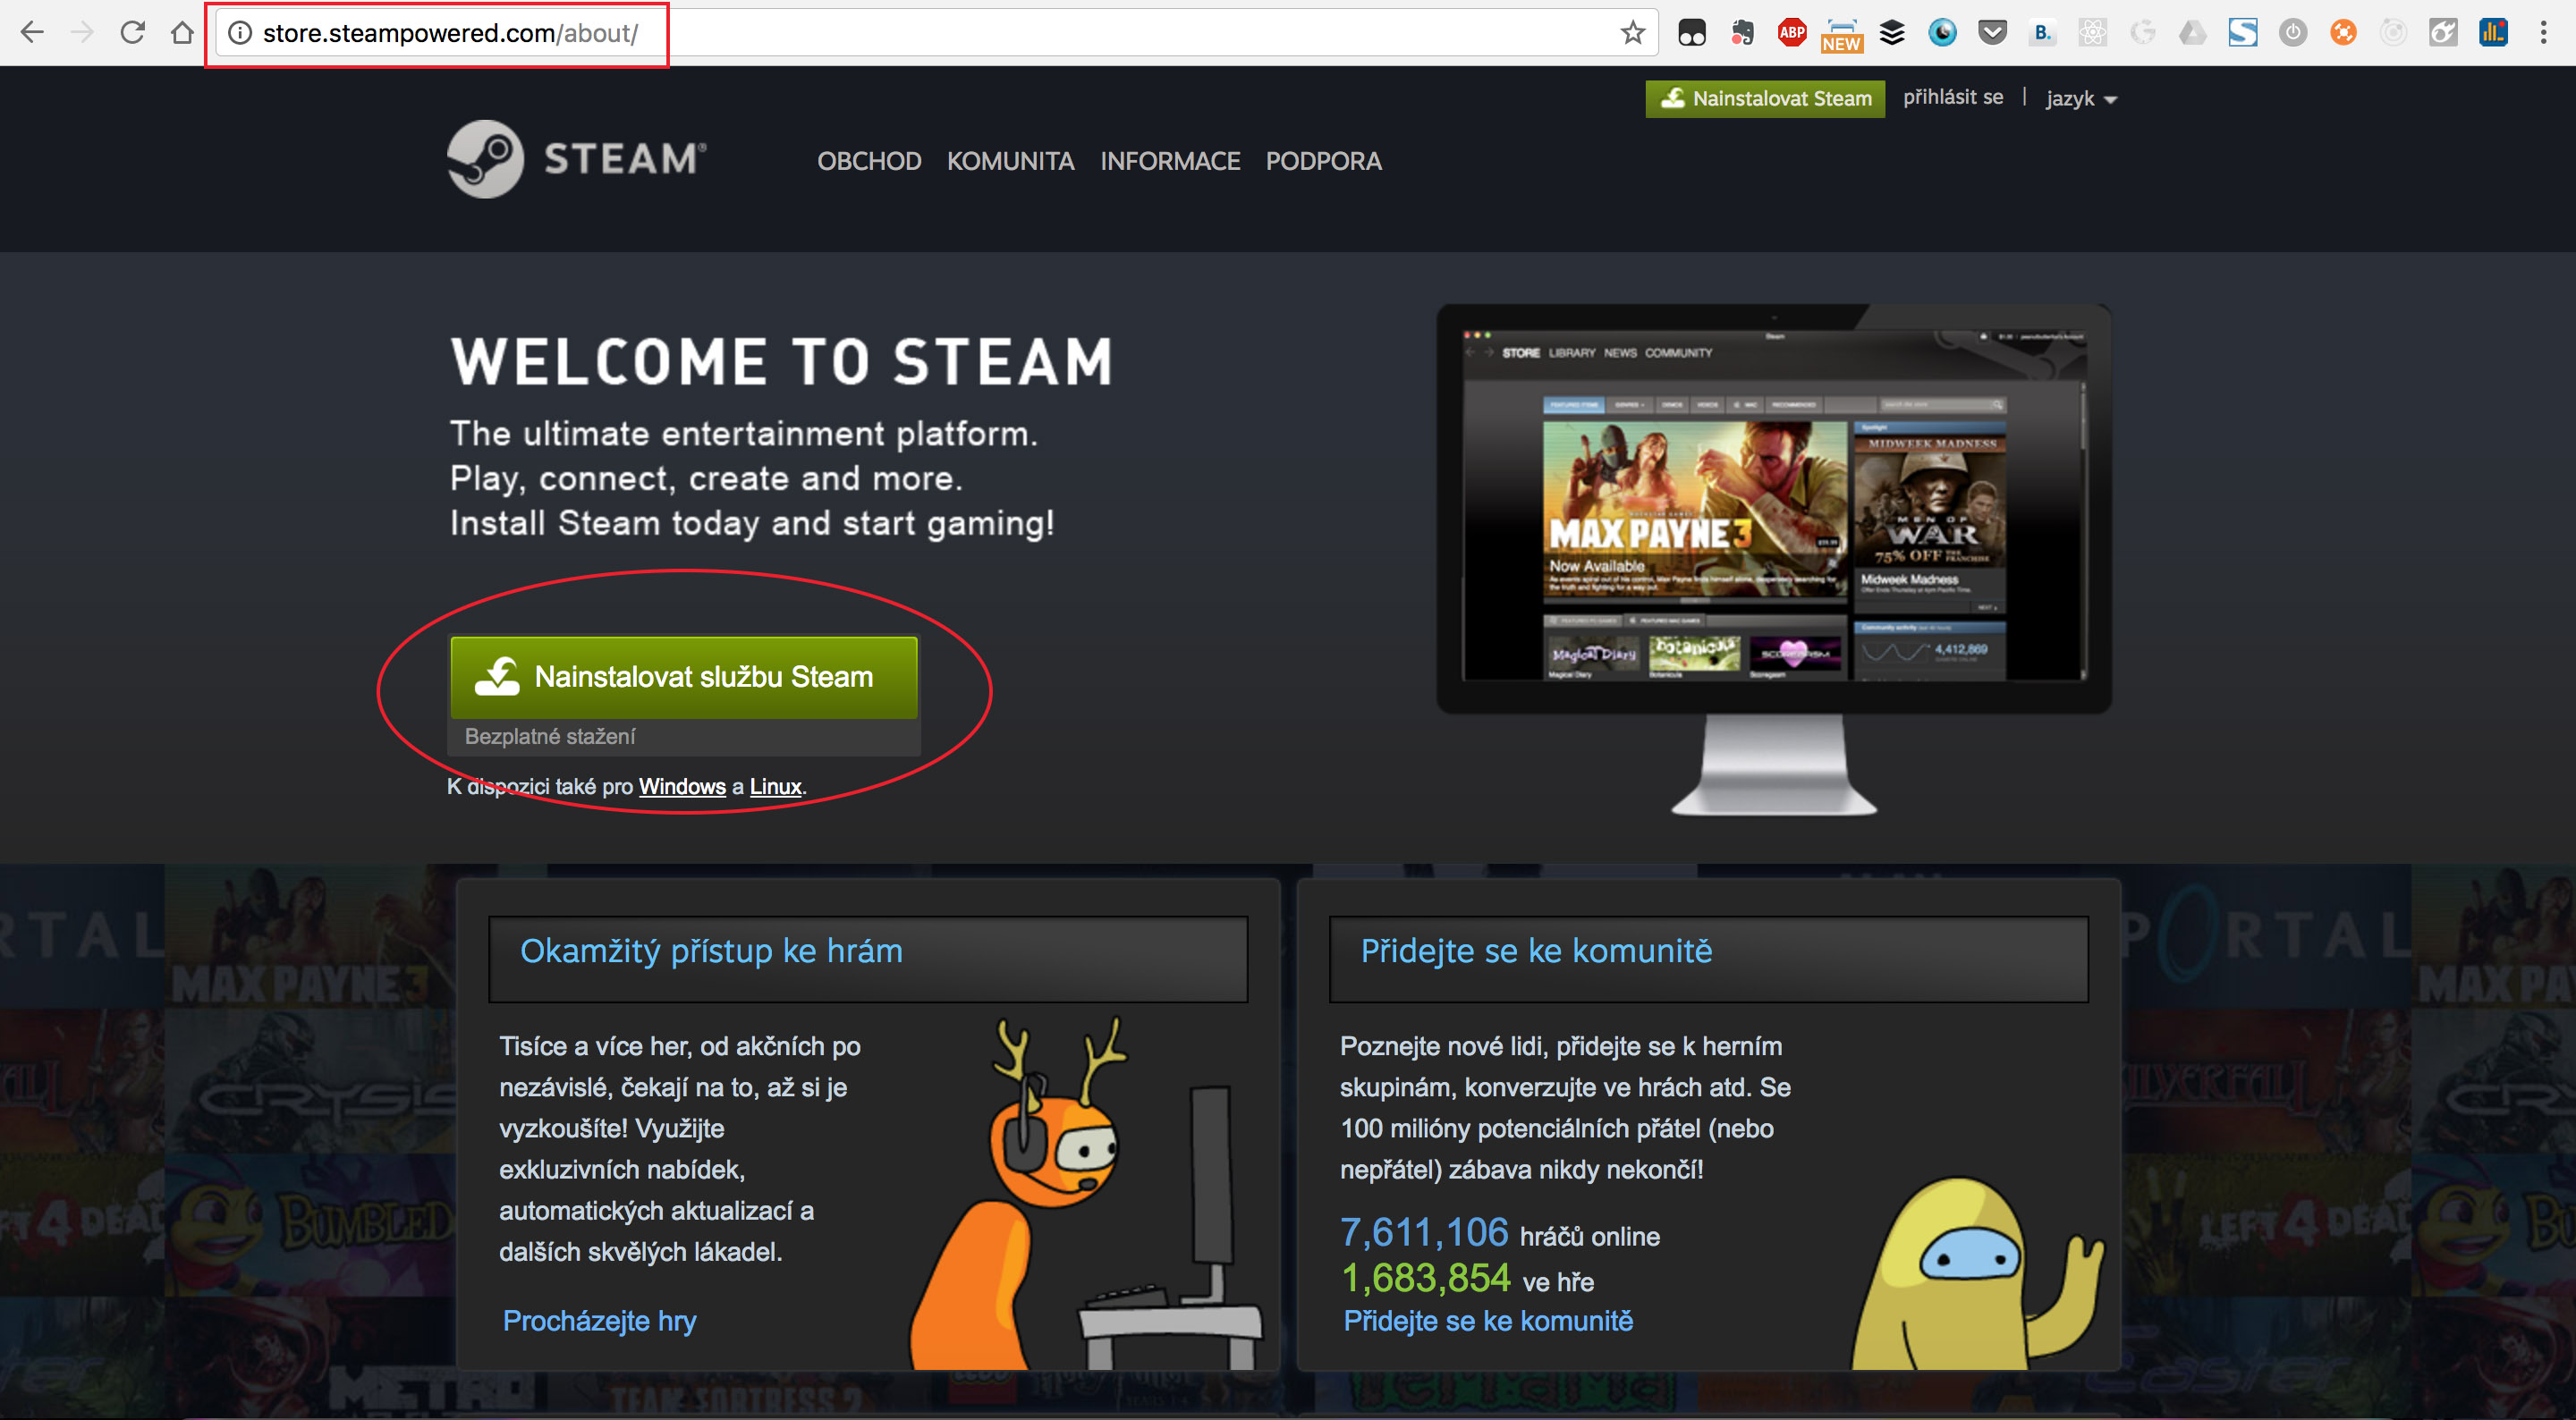
\includegraphics[width=0.8\textwidth]{steam}
\caption{Steam download page.}
\label{r:71}
\end{figure}

After Steam download is finished, you can open the installer and follow instructions.

For SteamVR, open installed Steam, navigate to \textsf{Library} and search for "steamvr". It should find the installer and show it in list view under \textsf{Tools}. Clicking on it will show a button in the right panel. Click on it to start SteamVR download, installation will begin automatically afterwards.

\begin{figure}[ht!]
\centering
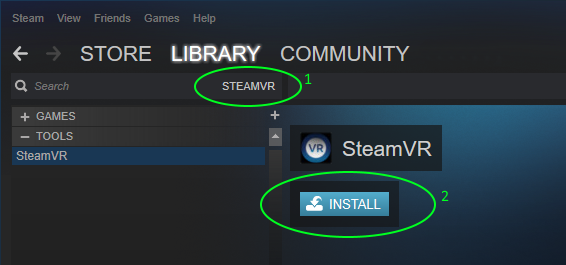
\includegraphics[width=0.8\textwidth]{steam-vr}
\caption{SteamVR installation button.}
\label{r:72}
\end{figure}

\newpage
\subsubsection*{Room-scale tracking setup}
After SteamVR is installed, room setup window will pop up automatically. For MathworldVR to work correctly, you need to select \textsl{Room-Scale} option and follow the tutorial.

\begin{figure}[ht!]
\centering
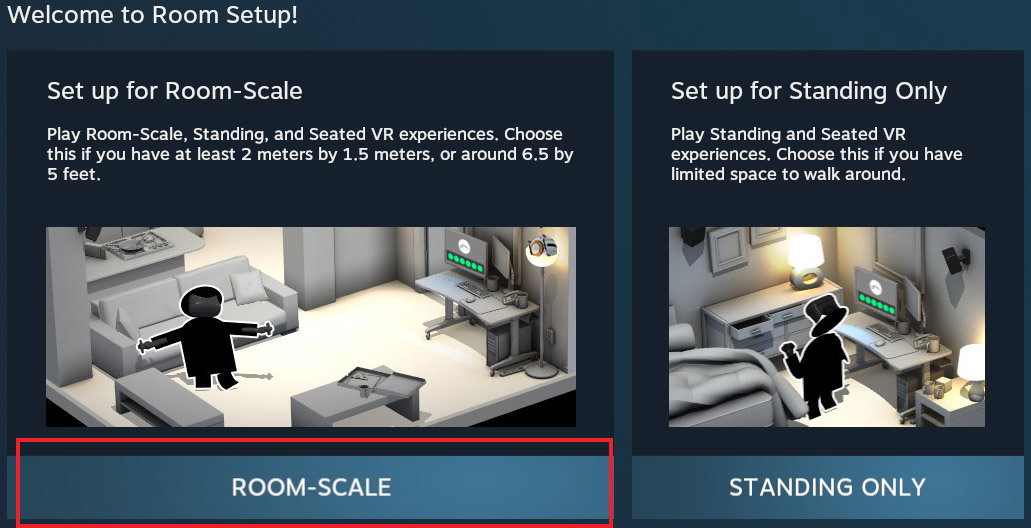
\includegraphics[width=0.9\textwidth]{room-scale-setup}
\caption{Room setup window.}
\label{r:73}
\end{figure}

\subsubsection*{WebVR-supported browser}
During the time of writing of this thesis, only Chromium (experimental version of Google Chrome) and Mozilla Firefox Nightly browsers supported WebVR API. We included Chromium browser with MathworldVR application on the appended CD.

Chromium doesn't need to be installed. To open it, user just needs to double-click on \texttt{chrome.exe} file. In order to enable access to the WebVR APIs in Chromium, user must select the "Enabled" option from the drop-down menu for the "Enable WebVR" flag (enter \texttt{chrome://flags/#enable-webvr} in the URL bar) and the "Gamepad Extensions" flag (enter \texttt{chrome://flags/#enable-gamepad-extensions} in the URL bar), or launch Chromium from the command line with the \texttt{--enable-webvr} and \texttt{--enable-gamepad-extensions} options.

\begin{figure}[ht!]
\centering
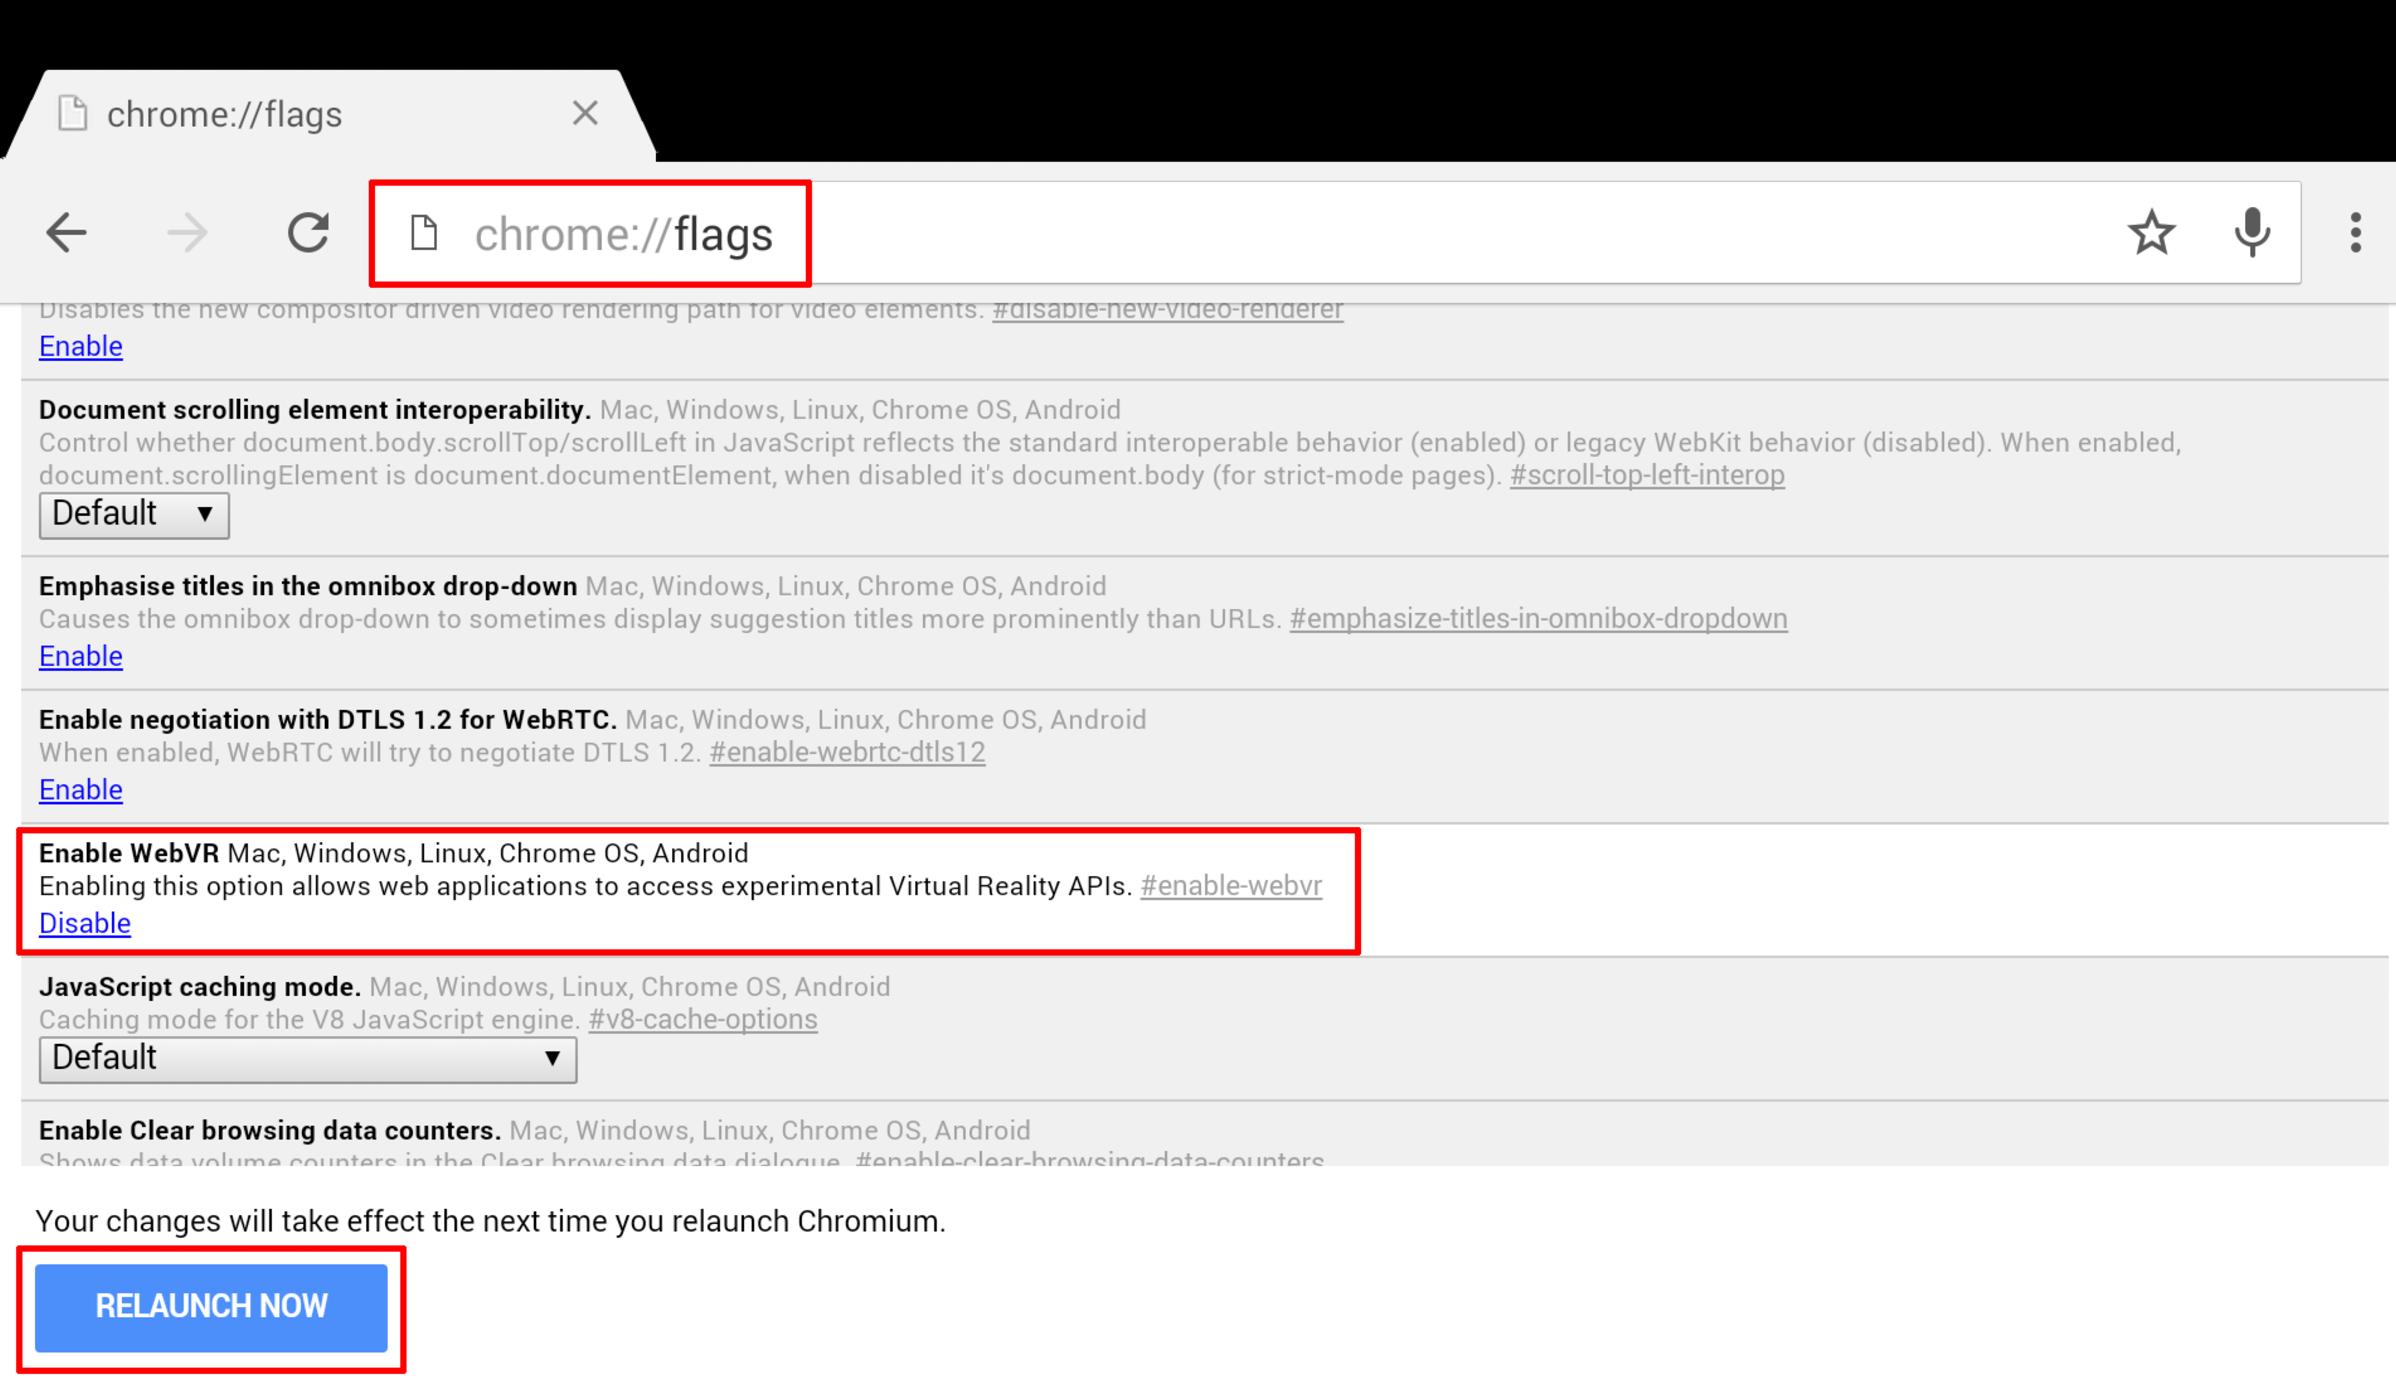
\includegraphics[width=0.9\textwidth]{chromium-flag}
\caption{Enabling the WebVR API in Chromium browser.}
\label{r:74}
\end{figure}


